% ============================================================
%  椰島 (Coconut Island) — 南島椰子主題 beamer theme
%  共用前導檔，供「說明」與「題解」兩份簡報 \input
%  以 XeLaTeX 編譯
% ============================================================
\documentclass[aspectratio=169,12pt]{beamer}

\usepackage{fontspec}
\usepackage{xeCJK}
\usepackage{tikz}
\usepackage{tcolorbox}
\tcbuselibrary{skins}
\usetikzlibrary{shapes.misc,arrows.meta}

% ---- 字型 ----
\setCJKmainfont{Heiti TC}
\setCJKsansfont{Heiti TC}
\setmonofont{JetBrainsMono Nerd Font Mono}
\setsansfont{JetBrainsMono Nerd Font}

% ---- 南島椰子色盤 ----
\definecolor{ocean}{HTML}{0F8B8D}     % 海洋藍綠
\definecolor{deepsea}{HTML}{0A5C5E}   % 深海
\definecolor{sand}{HTML}{F4E4C1}      % 沙灘
\definecolor{coconut}{HTML}{6B4226}   % 椰殼棕
\definecolor{leaf}{HTML}{3A7D44}      % 椰葉綠
\definecolor{sun}{HTML}{F2B705}       % 陽光黃
\definecolor{coral}{HTML}{E07A5F}     % 珊瑚橘
\definecolor{paperbg}{HTML}{FBF6EA}   % 米白底

% ---- Wordle 椰子三色 ----
\definecolor{wgreen}{HTML}{6AAA64}    % 熟椰：對的字母對的位置
\definecolor{wyellow}{HTML}{C9B458}   % 青椰：字母有但位置錯
\definecolor{wgray}{HTML}{787C7E}     % 空殼：沒這個字母

% ---- beamer 外觀 ----
\usetheme{default}
\setbeamertemplate{navigation symbols}{}
\setbeamercolor{background canvas}{bg=paperbg}
\setbeamercolor{frametitle}{bg=ocean,fg=white}
\setbeamercolor{title}{fg=deepsea}
\setbeamercolor{structure}{fg=ocean}
\setbeamercolor{normal text}{fg=coconut!90!black}
\setbeamercolor{itemize item}{fg=leaf}
\setbeamercolor{itemize subitem}{fg=ocean}
\setbeamerfont{frametitle}{series=\bfseries}
\setbeamertemplate{itemize item}{\textcolor{leaf}{\textbf{\textbullet}}}
\setbeamertemplate{itemize subitem}{\textcolor{ocean}{--}}

% 圓角的標題列
\setbeamertemplate{frametitle}{%
  \vspace{0.3em}%
  \begin{beamercolorbox}[wd=\paperwidth,sep=0.45em,leftskip=0.6cm]{frametitle}%
    \textbf{\strut\insertframetitle}%
  \end{beamercolorbox}%
}

% ---- Wordle 方塊 ----
% \tile{顏色}{字母}
\newcommand{\tile}[2]{%
  \tikz[baseline=-0.55ex]{\node[fill=#1,text=white,minimum size=0.92cm,
    inner sep=0pt,font=\bfseries\Large,rounded corners=2pt]{#2};}}
% 一整列五格
\newcommand{\wordrow}[1]{\begin{tikzpicture}[baseline]#1\end{tikzpicture}}

% ---- 小提示框 ----
\newtcolorbox{leafbox}[1][]{%
  enhanced, colback=leaf!8, colframe=leaf, boxrule=1pt, arc=4pt,
  fonttitle=\bfseries, coltitle=white, colbacktitle=leaf, #1}
\newtcolorbox{sunbox}[1][]{%
  enhanced, colback=sun!12, colframe=sun!85!black, boxrule=1pt, arc=4pt,
  fonttitle=\bfseries, coltitle=coconut, colbacktitle=sun, #1}
\newtcolorbox{oceanbox}[1][]{%
  enhanced, colback=ocean!8, colframe=ocean, boxrule=1pt, arc=4pt,
  fonttitle=\bfseries, coltitle=white, colbacktitle=ocean, #1}

% ---- 椰子小圖示 (tikz 畫的椰子) ----
\newcommand{\coconuticon}[1][1]{%
  \begin{tikzpicture}[scale=#1]
    \fill[coconut] (0,0) circle (0.32);
    \fill[coconut!70!black] (-0.1,0.08) circle (0.045);
    \fill[coconut!70!black] (0.1,0.08) circle (0.045);
    \fill[coconut!70!black] (0,-0.05) circle (0.045);
  \end{tikzpicture}}

% ---- 樹根朝天的椰子樹（本年度主題）----
% 畫在原點 (0,0) 為地面，往上長；在 tikzpicture 裡用 scope 平移／縮放：
%   \begin{scope}[shift={(x,y)},scale=s] \upsidedowntree \end{scope}
\newcommand{\upsidedowntree}{%
  % 樹幹：從地面往上
  \draw[line width=3pt, coconut] (0,0)
    .. controls (0.2,0.6) and (-0.05,1.1) .. (0.08,1.55);
  % 樹根朝天：頂端往天空分岔
  \foreach \a/\len in {118/0.5,98/0.62,80/0.6,62/0.48,140/0.4,58/0.34}{
    \draw[line width=1.6pt, coconut!85!black]
      (0.08,1.55) -- ++({\len*cos(\a)},{\len*sin(\a)});}
  % 細根的小分岔
  \foreach \a/\len in {100/0.18,82/0.18,120/0.14,60/0.14}{
    \draw[line width=1pt, coconut!85!black]
      ({0.08+0.5*cos(\a)},{1.55+0.5*sin(\a)}) -- ++({\len*cos(\a+25)},{\len*sin(\a+25)});}
  % 椰葉朝下：從樹冠（下方）往外垂
  \foreach \a in {205,232,258,282,308,335}{
    \draw[line width=2pt, leaf] (0.08,0.55)
      .. controls ({0.08+0.5*cos(\a)},{0.55+0.45*sin(\a)})
         and ({0.08+1.0*cos(\a)},{0.25+0.3*sin(\a)})
      .. ({0.08+1.3*cos(\a)},{0.08});}
  % 椰子：掛在樹冠附近（下方）
  \fill[coconut] (-0.12,0.5) circle (0.12);
  \fill[coconut] (0.3,0.52) circle (0.12);
}



\title{椰島字謎}
\subtitle{題解}

\begin{document}

% ---------- 封面 ----------
{\setbeamertemplate{footline}{}
\begin{frame}[plain]
  \centering
  \vspace{0.7cm}
  {\Huge\bfseries\textcolor{deepsea}{椰子尋寶}}\\[0.2cm]
  {\LARGE\textcolor{ocean}{題解}}\\[0.6cm]
\end{frame}}

\begin{frame}{思考策略}
  \begin{itemize}
    \item 最直覺的策略：
    \item 在紙上標記哪些椰子還有可能是答案
    \item 每次猜測後把不可能的地方劃掉
  \end{itemize}
\end{frame}

\begin{frame}{思考策略}
  \begin{itemize}
    \item 「可能答案」的集合可以稱為\textbf{搜索空間}
    \item 進攻跟防守隊的目標？
    \item 進攻：讓搜索空間越小越好，也就是劃掉越多地方越好
    \item 防守：讓搜索空間越大越好，也就是進攻方劃掉越少地方越好
  \end{itemize}
\end{frame}

\begin{frame}{思考策略}
  從這個角度出發，防守者要怎麼設計策略？
  \centering
  \vspace{0.1em}
  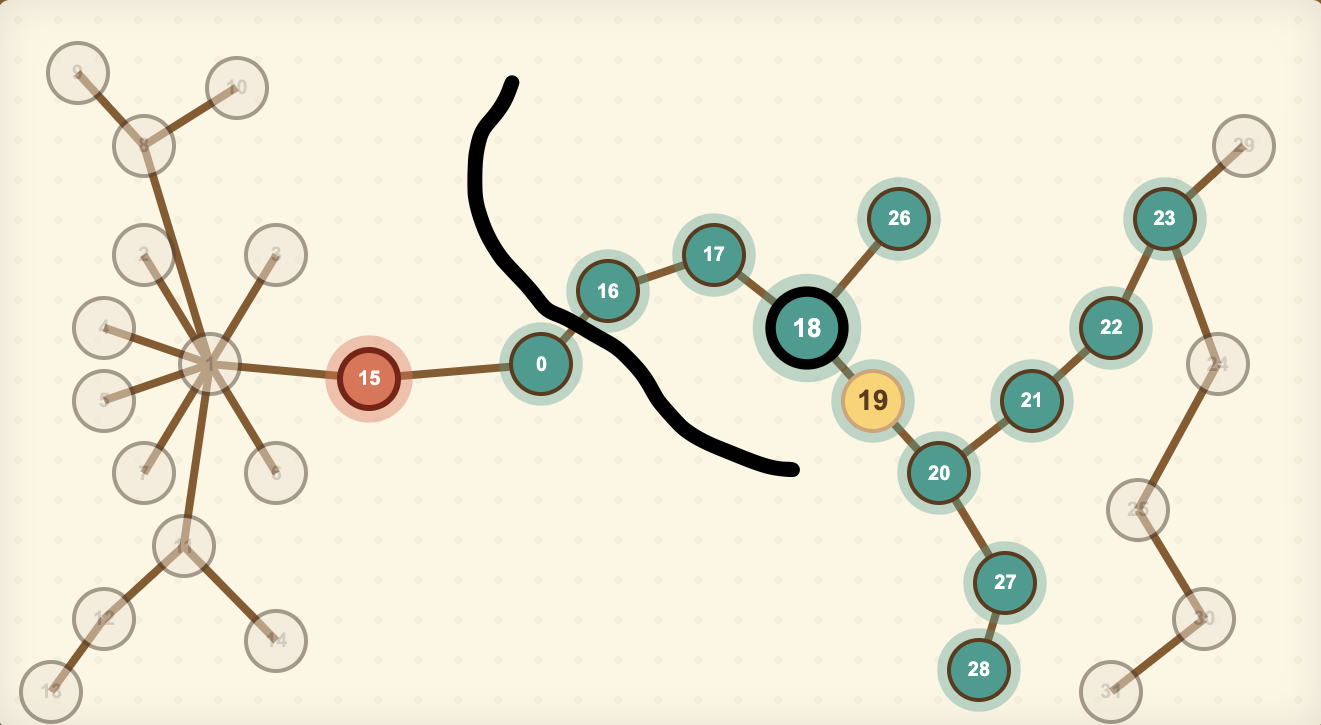
\includegraphics[width=0.75\textwidth]{edi_bad_def.png}\\[0.2em]
  {\footnotesize\textcolor{coconut!70!black}{
  如果猜 $18$，那黑線右邊的是還有可能的點}}
  \vspace{0.3em}

\end{frame}

\begin{frame}{思考策略}
  從這個角度出發，防守者要怎麼設計策略？
  \centering
  \vspace{0.1em}
  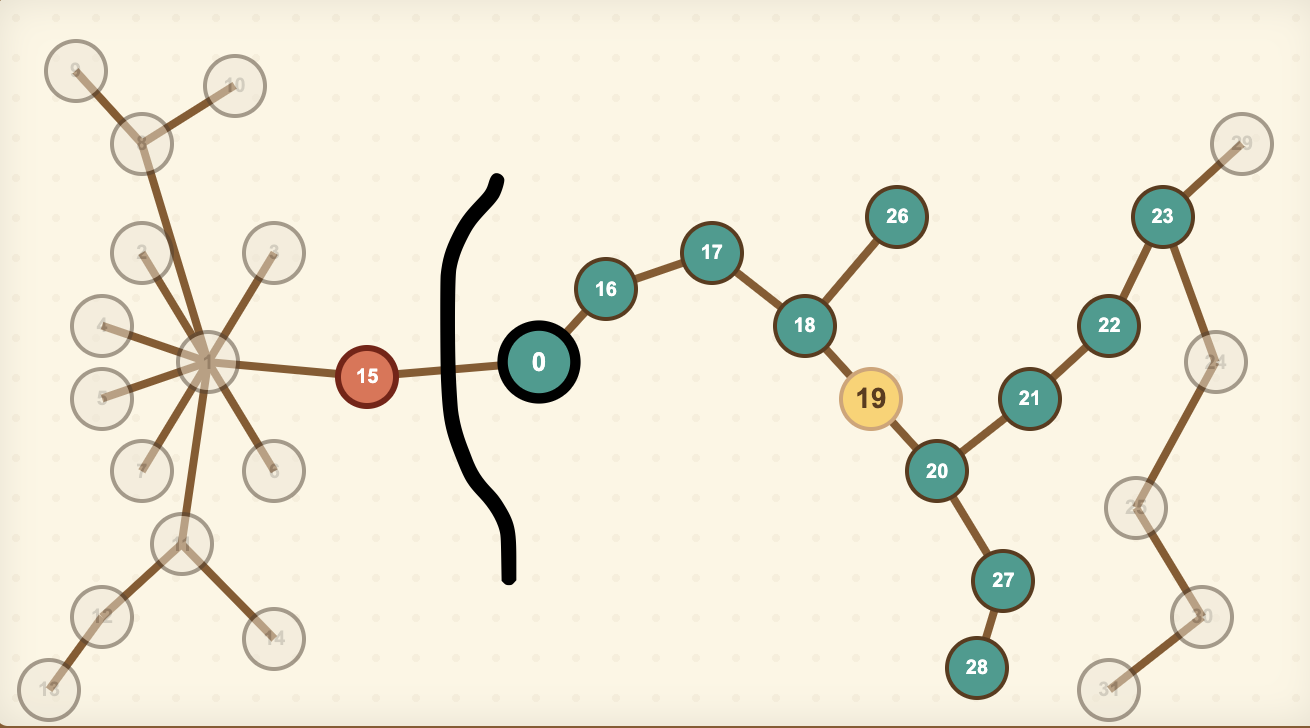
\includegraphics[width=0.75\textwidth]{edi_good_def.png}\\[0.2em]
  {\footnotesize\textcolor{coconut!70!black}{
  如果猜 $0$，那黑線右邊的是還有可能的點，數量比較多 $\Rightarrow$ 防守佔優勢}}
  \vspace{0.3em}

\end{frame}

\begin{frame}{思考策略}
  \begin{itemize}
    \item 可以看出，防守者每次的最佳策略都是回答某個進攻隊猜測的鄰居
    \item 這樣子會給對方最少\textbf{資訊}
    \item 知道防守者策略，就可以來思考進攻方要怎麼攻擊了
  \end{itemize}
\end{frame}

\begin{frame}{思考策略}
  假設進攻方猜 $23$，防守最好的策略就是告訴他\textbf{要往哪邊走}
  \centering
  \vspace{0.1em}
  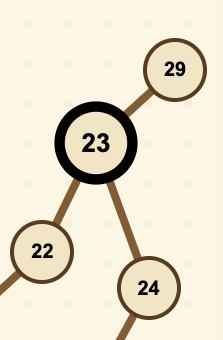
\includegraphics[width=0.27\textwidth]{att.png}\\[0.2em]
  {\footnotesize\textcolor{coconut!70!black}{
  也就是進攻方可以把兩個鄰居的點都劃掉，剩下一個鄰居的樹群}}
  \vspace{0.3em}
\end{frame}

\begin{frame}{思考策略}
  \begin{itemize}
    \item 因此，自然的想法就是猜\textbf{中間一點}的，因為這樣有機會把左邊所有人或是右邊所有人全部丟掉
    \item 我們想要選一個中間的點，使得說把它「拔掉」之後，剩下的「椰子島」最大的還是很小
    \item 可以證明說，如果都選最好的，那每次可以把至少一半的點刪掉
  \end{itemize}
\end{frame}

\begin{frame}{思考策略}
  \begin{itemize}
    \item 這樣子最壞情況是多少呢？
    \item 搜索空間大小變成 $1$ 就代表一定猜到了
    \item 一開始搜索空間大小是 $32$，每次至少除以 $2$
    \item 如果學過對數：$\frac{32}{2^x} \leq 1 \Rightarrow \log_{2} 32 \leq x \Rightarrow 5 \leq x$
    \item 最多猜 $5$ 次就成功了！
  \end{itemize}
\end{frame}

\begin{frame}{思考策略}
  \begin{itemize}
    \item 這種「把搜索空間變一半」的想法在演算法的世界很常見
    \item 像是大家可能有聽過「二分搜」，原理就是這樣
  \end{itemize}
\end{frame}

\begin{frame}{可以說謊？}
  \begin{itemize}
    \item 可以說謊怎麼辦？
    \item 一些策略：
    \begin{itemize}
      \item 可以說 2 次謊我就問同樣東西問 3 次
      \item 在紙上記錄每個點被「刪掉」幾次，被刪掉 3 次就確定不行了
      \item 猜看起來可以刪掉蠻多的東西的點
    \end{itemize}
  \end{itemize}
\end{frame}

\begin{frame}{可以說謊？}
  \begin{itemize}
    \item 可以說謊怎麼辦？
    \item 最佳策略（補充）：
    \begin{itemize}
      \item 我們還是想讓「搜索空間」每次變一半，但有些點已經被刪 3 次了，再刪他也沒用
    \end{itemize}
  \end{itemize}
\end{frame}

\begin{frame}{可以說謊？}
  \begin{itemize}
    \item 可以說謊怎麼辦？
    \item 最佳策略（補充）：
    \begin{itemize}
      \item 被刪兩次的點感覺比被刪一次的點還不可能很多
      \item 把「減 $1$」改成「除以 $2$」
    \end{itemize}
  \end{itemize}
\end{frame}

\begin{frame}{可以說謊？}
  \begin{itemize}
    \item 可以說謊怎麼辦？
    \item 最佳策略（補充）：
    \begin{itemize}
      \item 每個點上面寫一個數字，一開始為 $1$
      \item 每次一樣選「最中間」的地方
      \item 把「要說謊才能是寶藏」的地方都除以 $2$
      \item 每次「所有點的總和」都會被除以 $2$
    \end{itemize}
  \end{itemize}
\end{frame}

\begin{frame}{可以說謊？}
  \begin{itemize}
    \item 可以說謊怎麼辦？
    \item 最佳策略（補充）：
    \begin{itemize}
      \item 正確答案只能被說兩次謊，所以他上面的數字只會被除 $2$ 次 $\Rightarrow \geq \frac 1 4$
      \item 只要「所有點的總和」$\leq \frac 1 4$ 就可以確定最佳答案了！
      \item 一開始是 $32$，要變 $\leq \frac 1 4$，只要除以二 $7$ 次就變 $\frac 1 4 \Rightarrow$ 得到答案了
    \end{itemize}
  \end{itemize}
\end{frame}

\end{document}